% Run: arara -l *.tex to generate a log file (arara.log) of the compilation for traceability and debugging.
% Running -l instead of -v is also quicker to run.

% synctex: on - an input and output synchronization feature that allows navigation from source to typeset material and vice versa.
% interaction: nonstopmode - Tex does not request input after serious errors but stops altogether.
% shell: yes - shell escape to add compilation parameters.

% arara: pdflatex: { synctex: on, interaction: nonstopmode, shell: yes }
% arara: makeglossaries
% arara: biber
% arara: pdflatex: { synctex: on, interaction: nonstopmode, shell: yes }
% arara: pdflatex: { synctex: on, interaction: nonstopmode, shell: yes }


% article - the document class.
% hidelinks - removes the borders around clickable cross-references and hyperlinks
% 12pt - font size of the document.
% a4paper - paper size and format.

% draft - speeds up typesetting, because figures are not loaded, just indicated by a frame.
% Hyperref items will only be displayed without the functionality.
% The complication process using the "draft" option is quicker to run.
% Delete the "draft" option or replace it with "final" in the final document version.

% Other options include: twocolumn, landscape, titlepage, openright, and openany.
\documentclass[final, hidelinks, 12pt, a4paper]{article}

% Solves the error which occurs when user's packages have allocated too many streams - Tex fixed limit is 16
\usepackage{morewrites}

% Provides a wider range of input encodings using standard mappings
\usepackage[utf8]{inputenc}

% Constructs headers and footers
\usepackage{fancyhdr}

% Provides a key-value interface for optional arguments to the \includegraphics command
\usepackage{graphicx}

% Provides various features to facilitate writing math formulas and to improve the typographical quality of their output
\usepackage{amsmath}
\usepackage{amssymb}

% Provides many ways to customize the captions in floating environments like figure and table, and cooperates with many other packages
\usepackage{caption}

% Allows the use of sub-caption
\usepackage{subcaption}

% Draws diagonal lines and arrows with limits through parts of maths formulas
% thicklines - provides heavier lines and arrows
% makeroom - increases the horizontal spacing to make room for the cancellation value
\usepackage[thicklines, makeroom]{cancel}

% Provides both foreground and background color management. Also, provides easy driver-independent access to several kinds of color tints, shades, tones, and mixes of arbitrary colors
% dvipsnames - makes the color names for the driver dvips available.
\usepackage[dvipsnames]{xcolor}

% Supports common layouts for tabular column heads in whole documents, based on one-column tabular environment
\usepackage{makecell}

% Provides a simple LaTeX interface for the processing of files with comma separated values (CSV)
\usepackage{csvsimple}

% Defines a multicols environment which typesets text in multiple columns (up to a max. of 10), and (by default) balances the end of each column at the end of the environment
\usepackage{multicol}

% Provides additional features to existing packages and a consistent interface
\usepackage{siunitx}

% Produces hypertext links
% pdftex - tex variant that writes PDF directly
% breaklinks - allow links to break over lines by making links over multiple lines into PDF links to the same to the same target
% bookmarks - A set of Acrobat bookmarks are written, in a manner similar to the table of contents, requiring two passes of LATEX. 
% Some postprocessing of the bookmark file (file extension .out) may be needed to translate LATEX codes, since bookmarks must be written in PDFEncoding.
% To aid this process, the .out file is not rewritten by LATEX if it is edited to contain a line \let\WriteBookmarks\relax
% bookmarksopen - If Acrobat bookmarks are requested, show them with all the subtrees expanded.
% bookmarksnumbered - If Acrobat bookmarks are requested, include section numbers.
% pdfmenubar - make PDF viewer's menu bar visible.
\usepackage[bookmarks, bookmarksnumbered, bookmarksopen, breaklinks, pdftex, linktoc=all, pdfmenubar]{hyperref}
%\let\WriteBookmarks\relax
% Setting the title, author, and creator of the PDF
\hypersetup{pdftitle={SYSYC4005 - Milestone 2 Report},
            pdfauthor={Ghassan Arnouk},
            pdfcreator={Ghassan Arnouk}}

% Enables the user to typeset programs (programming code) within Latex. The source code is read directly and not processed 
\usepackage{listings}

% References the number of pages in your Latex document through the introduction of a new label which can be referenced to give a reference to the last page of a document
\usepackage{lastpage}



% Selectively include/exclude pieces of text, allowing the user to define new, separately controlled, comment version
\usepackage{comment}

% [In Progress]
% Must be inserted after the biblatex package to overwrite biblatex url handling - for consistency
\usepackage{xurl}

% Moves the typesetting position from the left margin of the paragraph
\usepackage{tabto}

% Provides user control over the layout of the three basic list environments: enumerate, itemize, and description
\usepackage{enumerate}

% Manages culturally-determined typographical (and other) rules for a wide range of languages.
% Language specified is English 
\usepackage[english]{babel}

% Provides advanced facilities for inline and display quotations
\usepackage{csquotes}

% Include code blocks with syntax highlighting
\usepackage{minted}

% Provides user with control over the spacing between the lines of the document
% However, footnotes, figures, and tables will still be single spaced.
% Must be place before \begin{document}
% \doublespacing
% \singlespacing
% \onehalfspacing
% \setstretch{1.25}
\usepackage{setspace}

% Provides various ways of formatting the titles of appendices. Also (sub)appendices environments are provided.
% titletoc - adds a name (e.g. Appendix) before each appendix listed in the ToC.
% page - puts a title (e.g. Appendices) into the document at the point where the appendices environment is begun.
\usepackage[page]{appendix}

% Provides tools to generate plots and labeled axes easily
\usepackage{tikz}
\usepackage{pgfplots}
\usepgfplotslibrary{groupplots}


% Provides an easy and flexible user interface to customize page layout, implementing auto-centering and auto-balancing mechanisms so that the users have only to give the least description for the page layout.
% includeheadfoot - sets both includehead and includefoot to true.
% margin - sets the margins of the Latex document.
% Other options:
% twoside - switches on twoside mode with left and right margins swapped on verso pages.
% asymmetric - implements a twosided layout in which margins are not swapped on alternate pages (by
% setting \oddsidemargin to \evensidemargin + bindingoffset) and in which the
% marginal notes stay always on the same side. 
% This option can be used as an alternative to the twoside option.
\usepackage[margin=1in, includeheadfoot]{geometry}

% Formatting bibliography.
% Bibliography style=ieee.
% backend=biber - the backend of biblatex used to transfer data from source files to the Latex code.
\usepackage[style=ieee, backend=biber]{biblatex}

% Supports acronyms and multiple glossaries, and has provision for operation in several languages.
\usepackage[debug, toc, section=section, acronym, symbols]{glossaries} 

% Allows the use and import of markdown files.
% codeSpans - Enable the code span syntax.
% [In Progress]
\usepackage[fencedCode, inlineFootnotes, citations, definitionLists, hashEnumerators, smartEllipses, hybrid, codeSpans]{markdown}


% Fixes package fancyhdr Warning: \heatheight is too small (12.0pt)
\setlength{\headheight}{14.49998pt}
% Makes \topmargin smaller to compensate the change introduced in the previous line
\addtolength{\topmargin}{-2.49998pt}


% A path to the images directory to be imported in the tex document
\graphicspath{{./Imports/Images/}}

% A path to the bibliography directory to be imported in the tex document
\addbibresource[location=local]{./Imports/Bibliography/accelerators.bib}

% Add constants list using glossary
\newglossary[cgls]{constants}{cstog}{cstig}{Constants}
% Alphabetize glossary and acronyms list
\makeglossaries


% Code spanning over multiple pages using the minted package
% The new environment name is `code`
\newenvironment{code}{\captionsetup{type=listing}}{}


% Changes the page number of titlepage, toc, lot, lof, and lol to roman
\pagenumbering{roman}


% A new command for less cramped nested fractions
\newcommand\ddfrac[2]{\frac{\displaystyle #1}{\displaystyle #2}}

% A new command for colored cancellation marks
\renewcommand{\CancelColor}{\color{red}}

% Define the background colors of a block of code
\definecolor{bg}{rgb}{0.95,0.95,0.95}

% Use the line below to bold \SI{}{} commands
\sisetup{detect-all=true}

% A special delimiter for bits of code that should be evaluated
\lstset{escapeinside={<}{>}}

% A customized counter to keep track of '<++>TEXT'
%\newcounter{<++>VARIABLE}
%\newcommand\<++>THENEWCOMMAND{\stepcounter{<++>VARIABLE}TEXT \the<++>VARIABLE}

% Changes the heading of the list of listings from 'Listings' to anything the user desires
%\renewcommand{\lstlistlistingname}{<name>}



%%%%%%%%%%%%%%%%%%%% Glossaries %%%%%%%%%%%%%%%%%%%%
% Glossaries go here



%%%%%%%%%%%%%%%%%%%%% Acronyms %%%%%%%%%%%%%%%%%%%%%
% Acronyms go here
\newglossaryentry{iqr}
{
    type=\acronymtype,
    name={IQR},
    description={InterQuartile Range},
}
\newglossaryentry{q3}
{
    type=\acronymtype,
    name={Q3},
    description={Third Quartile},
    first={Third Quartile (Q3)}% \glsadd{<++>}},
    % see=[Glossary:]{<++>}
}
\newglossaryentry{q1}
{
    type=\acronymtype,
    name={Q1},
    description={First Quartile},
    first={First Quartile (Q1)}% \glsadd{<++>}},
    % see=[Glossary:]{<++>}
}
\newglossaryentry{n}
{
    type=\acronymtype,
    name={n},
    description={Total Number of Data Points},
}
\newglossaryentry{qq}
{
    type=\acronymtype,
    name={Q-Q},
    description={Quantile-Quantile},
    first={Quantile-Quantile (Q-Q)}% \glsadd{<++>}},
    % see=[Glossary:]{<++>}
}





%%%%%%%%%%%%%%%%%%%%% Symbols %%%%%%%%%%%%%%%%%%%%%%
% Symbols go here



%%%%%%%%%%%%%%%%%%%% Constants %%%%%%%%%%%%%%%%%%%%%
% Constants go here




% The document starts here!!
\begin{document}
    \begin{titlepage}
        \begin{center}
        	\vspace{1cm}
            % Lab report title
            {\LARGE{\bfseries Milestone 2 Report}}\\

            % Student name & student no.
            \vspace{1.5cm}
            {\large {\bfseries Ghassan Arnouk}}\\
            {\large {\bfseries 101078550}}\\
            \vspace{0.2cm}
            {\large {\bfseries Kareem El-Assad}}\\
            {\large {\bfseries 101107739}}\\
            \vspace{0.2cm}
            {\large {\bfseries Evan Lloyd}}\\
            {\large {\bfseries 101108670}}\\
            
            % Course code, Term, Lab # Report
            \vspace{1cm}
            {\large SYSC 4005A}\\
            {\large Winter 2023}\\
            {\large Group 49}\\


            % Instructor
            \vspace{2cm}
            {\bfseries Instructor:} Prof. Changcheng Huang\\

            % Day submitted
            \vspace{1cm}
            {\bfseries Day Submitted:} \today\\
    	\end{center}
    \end{titlepage} 


    % Prints table of content, update and maintain it automatically
    \tableofcontents
    \clearpage

    % Prints list of tables, update and maintain it automatically
    \listoftables
    \clearpage
    
    % Prints list of figures, update and maintain it automatically
    \listoffigures
    \clearpage

    % Prints list of listings, update and maintain it automatically
    \listoflistings
    \clearpage


    % Defines page style, header, and footer
    \pagestyle{fancy}
    % Student name & student no.
    \lhead{Group 49}
    % Lab report title
    \rhead{Milestone 2 Report}
    \rfoot{Page \thepage\ of \pageref{LastPage}} 
    % Hides page number in the middle of the footer
    \cfoot{}

    % Changes the page numbering of the document back to Arabic
    \pagenumbering{arabic}


    % First section goes here
    \section{Data Collection \& Input Modelling}
    \subsection{Distributions}
    \label{sct:distributions}
    The histograms of the provided data are shown in Fig. \ref{fig:histo}.
    \begin{figure}[htbp]
        \centering
        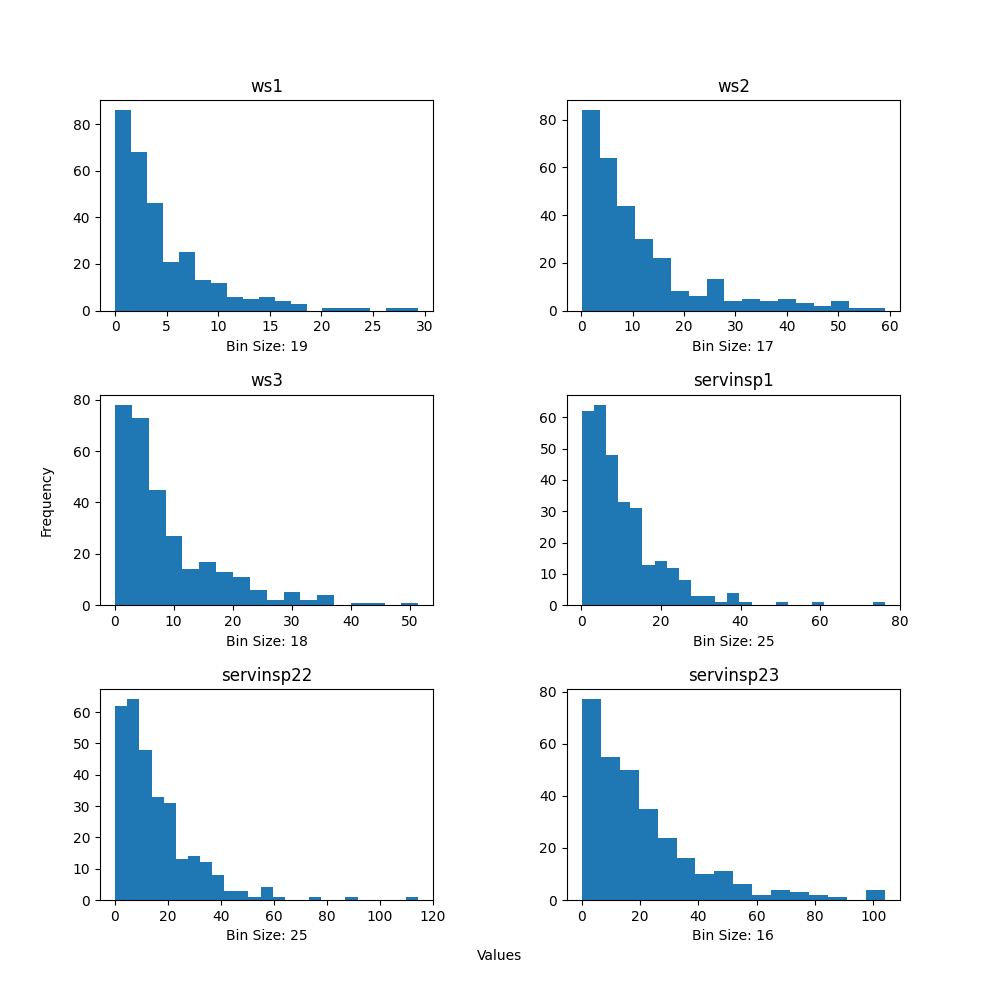
\includegraphics[width=\linewidth]{data_histogram_plots.png}
        \caption{Histograms of the provided data}
        \label{fig:histo}
    \end{figure}
    \clearpage
    \subsubsection{Bin Size}
    \label{sssct:binSize}
    As shown in listing \ref{lst:plotHistograms}, the bin size is calculated using the Freedman-Diaconis rule with the following equation \cite{acc:binSize}:
    \begin{align}
        W = \frac{2 \gls{iqr}}{\gls{n}^{\frac{1}{3}}}
        \label{eqt:binWidth}
    \end{align}
    The \gls{iqr} is calculated by subtracting the \gls{q1} value from the \gls{q3} value using the following equation:
    \begin{align}
        \gls{iqr} = \gls{q3} - \gls{q1}
        \label{eqt:iqrMath}
    \end{align}
    The bin size used on the provided data, to generate the histograms, is as follows:
    \begin{itemize}
        \item $ws_1 \rightarrow 19$
        \item $ws_2 \rightarrow 17$
        \item $ws_3 \rightarrow 18$
        \item $servinsp_1 \rightarrow 25$
        \item $servinsp_2 \rightarrow 25$
        \item $servinsp_3 \rightarrow 16$
    \end{itemize}


    \subsubsection{Choice of Distribution}
    \label{sssct:choiceDistribution}
    Using the plots shown in Figure \ref{fig:histo}, the histograms for the 6 data sets are identified as follows:
    \begin{itemize}
        \item $ws_1 \rightarrow$ Exponential
        \item $ws_2 \rightarrow$ Exponential
        \item $ws_3 \rightarrow$ Exponential
        \item $servinsp_1 \rightarrow$ Exponential
        \item $servinsp_2 \rightarrow$ Exponential
        \item $servinsp_3 \rightarrow$ Exponential
    \end{itemize}
    \subsubsection{Discussion}
    \label{sssct:discussion}
    Choosing a proper bin size is an essential key to creating histograms.
    The bin size also plays a big role in visualizing and interpreting the data.
    A good bin size for a histogram requires a balance between accurate representation of the data as well as clear and informative visual display.\\\\
    The ideal bin size varies depending on several factors such as: size of the data set, range of the data, distribution of the data, and lastly, the purpose of the histogram.\\\\
    For the size of the data set, a larger data set have more variation and may require a smaller bin size to capture the detail and structure of the data.
    Considering the range of the data, if the range is very large, a larger bin size may be required to avoid oversimplification of the data.
    In addition, if the goal of the histogram is to compare trends or how best the data fit a model, then a smaller bin size may be required to detect small differences.\\\\
    Using the shapes of the generated histograms, shown in Fig. \ref{fig:histo}, it is observed that $ws_1$, $ws_2$, and $ws_3$ follow an exponential distribution.
    The exponential distribution is often used in reliability analysis, where it used to model the time until a failure occurs.
    Generally, it is used to model waiting times.
    For instance, modelling the time between generating different products (P1, P2, P3) assuming the events of generating those products occur randomly and independently at a constant rate.\\\\
    Similarly, $servinsp_1$, $servinsp_2$, and $servinsp_3$ also follow an exponential distribution, as shown in Fig. \ref{fig:histo}.
    The main advantage of using the exponential distribution for the service time of inspectors is that the probability of the inspection occurring and passing the inspection is independent of how much time has gone by since the last occurrence of the inspection.
    \clearpage
    \subsection{Q-Q Plotting}
    \label{sct:qqPlot}
    \subsubsection{Histogram is not enough}
    \label{sssct:histoNotEnough}
    An important factor that is a limitation to histograms is the sensitivity to the choice of the bin size.
    If the bin size is too large, important details about the histogram may be lost due to oversimplification of the data.
    On the other hand, if the bind size is too small, the histogram can become more complex and difficult to comprehend.
    \subsubsection{Theory Behind Q-Q Plotting}
    \label{sssct:theoryQQ}
    The objective of \gls{qq} plot is to determine if two data sets come from the same distribution \cite{acc:qq}.
    Furthermore, constructing a \gls{qq} plot is done by plotting the first data set's quantiles against the second data set's quantiles.
    When observing a generated \gls{qq} plot, it is seen that the points match up a straight line indicating that the quantifies match \cite{acc:qq}.
    While the straight line plotted is not an essential component of a \gls{qq} plot, it allows a visual representation of where the points should line up \cite{acc:qq}.
    \subsubsection{Q-Q Plots}
    \label{sssct:qqPLOTS}
    {\bfseries Sample Calculations}\\\\
    Note that all the calculations were completed using listing \ref{lst:qqplotspy}.
    However, the steps below outlined to demonstrate the process and the calculations performed.
    \begin{description}
        \item {\bfseries Step 1:} Ordering the data set from smallest to largest
        \item {\bfseries Step 2:} Drawing a normal distribution curve
        \item {\bfseries Step 3:} Finding the z-value (cuttoff point) for each segment
        \item {\bfseries Step 4:} Plotting the data set values (from step 1) against the normal distribution cuttoff points (from step 3)
    \end{description}
    \clearpage
    \noindent The \gls{qq} plots of the provided data are shown in Fig. \ref{fig:qqPlotData}.
    \begin{figure}[htbp]
        \centering
        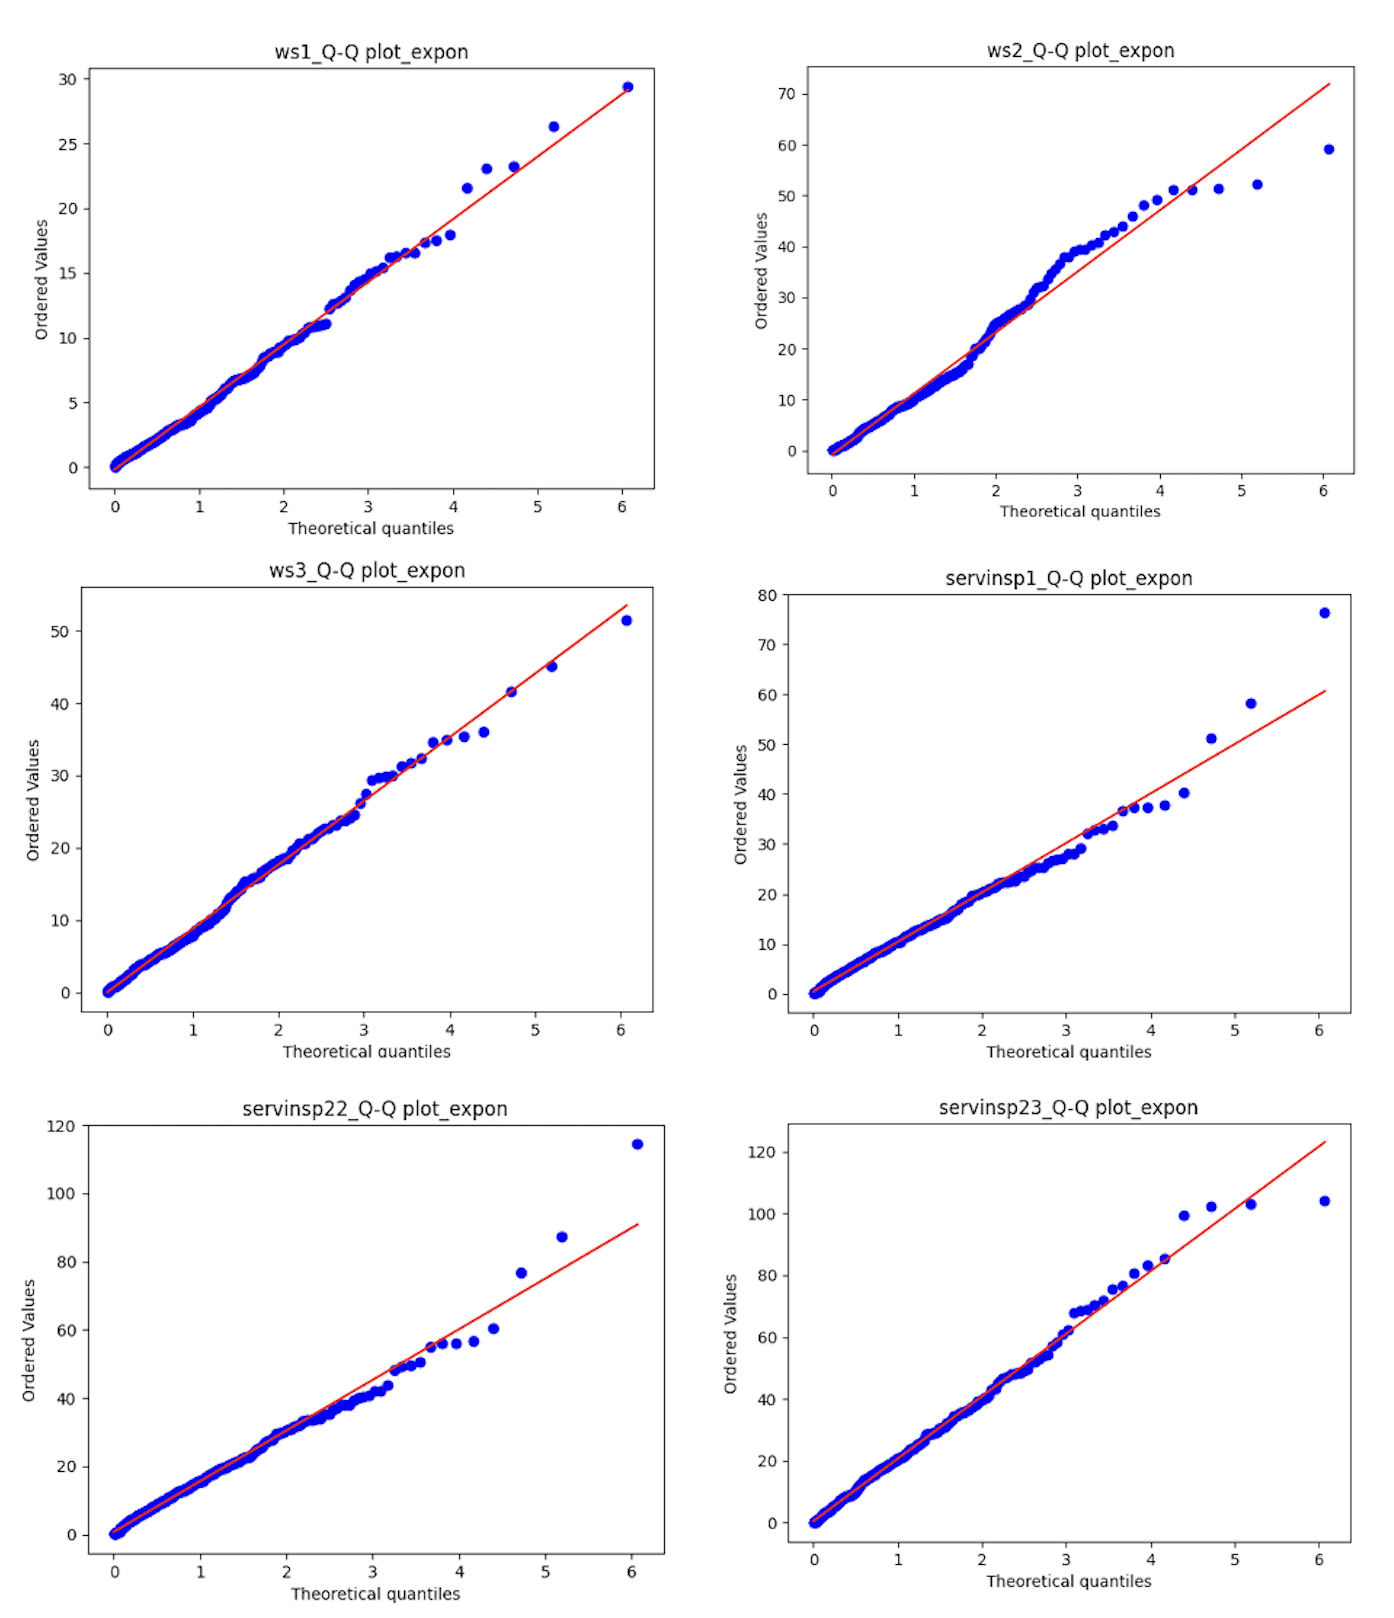
\includegraphics[width=0.85\linewidth]{qqPlots.png}
        \caption{Q-Q plots of the provided data}
        \label{fig:qqPlotData}
    \end{figure}
    \clearpage
    \subsubsection{Non-linearity at Certain Points}
    \label{sssct:nonLinPoints}
    The non-linear points of on the \gls{qq} plot indicates the differences in the shape of the distributions (how not similar the distributions are).
    However, as shown in Fig. \ref{fig:qqPlotData}, the majority of the individual \gls{qq} plots are linear and therefore, the non-linearity is correlated to the differences in the spread of the data as well as the presence of outliers in the data sets.
    \subsubsection{Conclusion}
    \label{sssct:qqConclusion}
    A bin size for the histogram was chosen and calculated using the Freedman-Diaconis rule due its relevance and easy of use.
    Appropriate bin size values were generated aiding in generating various histograms.
    The histograms followed an exponential distribution matching context of the data (the purpose the data serves).
    Additionally, \gls{qq} plots were generated which was linear for the most part verifying the results obtained from the histograms.
    The \gls{qq} plots showed non-linearity at certain points due to the spread of the data and the presence of outliers.
    The exponential distribution was a good choice for the distribution of the data sets as it was verified by the resulted \gls{qq} plots.
    \clearpage
    \subsection{Chi-Square}
    \label{sct:chiSquare}
    \subsubsection{Theory Behind Chi-Square Test}
    \label{sssct:theoryChiSq}
    The Chi-Square test is a hypothesis test that is used to determine whether there is a relationship between two categorical variables or not \cite{acc:chiTh}.
The objective of the Chi-Square test is to compare the observed frequency distribution of a categorical variable with the expected frequency distribution of the same variable \cite{acc:chiTh}.
    \clearpage
    \section{Input Generation}
    \label{sct:inputGen}
    \subsection{Creating and Testing RNG}
    \label{ssct:testRNG}
    \subsubsection{Discussion of Theory}
    \label{sssct:rngTh}
    To run our simulation accurately, it is required for wait times to be generated.
    For our simulation to be accurate these wait times must be based on historical data from the actual system that we are simulating.
    In the case of our project, we are completing input modeling on the time it takes for our inspections to complete and the time it takes for our workstations to completing assembly.
    We then use the data collected during our input modeling in combination with a random number generator to generate wait times for our simulation.
    For the simulation to accurately reflect the actual system these values must be values that could be recorded by the actual system and in a similar distribution to the historical data.
    Using arbitrary random values for our wait times would make it so that our simulation does not reflect the actual system.\\\\
The random numbers we generate should be uniform and independent. For random numbers to be uniform the generated values should be evenly distributed between 0 and our max value, usually 1.
    If our values were not uniform, the numbers would be skewed to certain values.
    This would result in our simulation being inaccurate since the generated wait times would not reflect the actual wait times of the system.
    For random numbers to be independent, the probability of generating a value should be independent of previously generated values.
    This ensures that the values being generated are truly random and not just based on previous values.\\\\
    An issue we face with simulation is a computer is unable to generate truly random values.
    A computer is a completely deterministic system meaning there is no randomness involved.
    Using certain methods, computers are able to generate pseudo random numbers.\\\\
    Two methods for pseudo random number generation are the linear congruential method and combined linear congruential generators.
    Combined linear congruential generators use multiple linear congruential methods that don’t have an increment value, also known as multiplicative congruential generators.
    The advantage of combined linear congruential generators is that they have a longer period (the number of values generated before the generator repeats).
    For our purpose the linear congruential method will provide us with a long enough period.\\\\
    To generate a sequence of pseudo random number using the linear congruential method, the following formula is used:
    \begin{align}
        x_{i+1} = (aX_i + c) mod\ m
        \label{eqt:lincon}
    \end{align}
    To ensure that our function has maximum density and period, we must choose appropriate values for $a$, $X_i$, $c$ and $m$.
    The values used were L'Ecuyer's suggested values for an RNG \cite{acc:eu}.
    The values that were chosen are m = 32749, a = 9515, c = 0 and x.\\\\
    As shown in \ref{lst:ranNumGen}, the function generateValue uses the chosen seed, a, c and m values to generate a series of pseudo random variables.
    The main function runs it 200 time and prints the results.
    \begin{figure}[htbp]
        \centering
        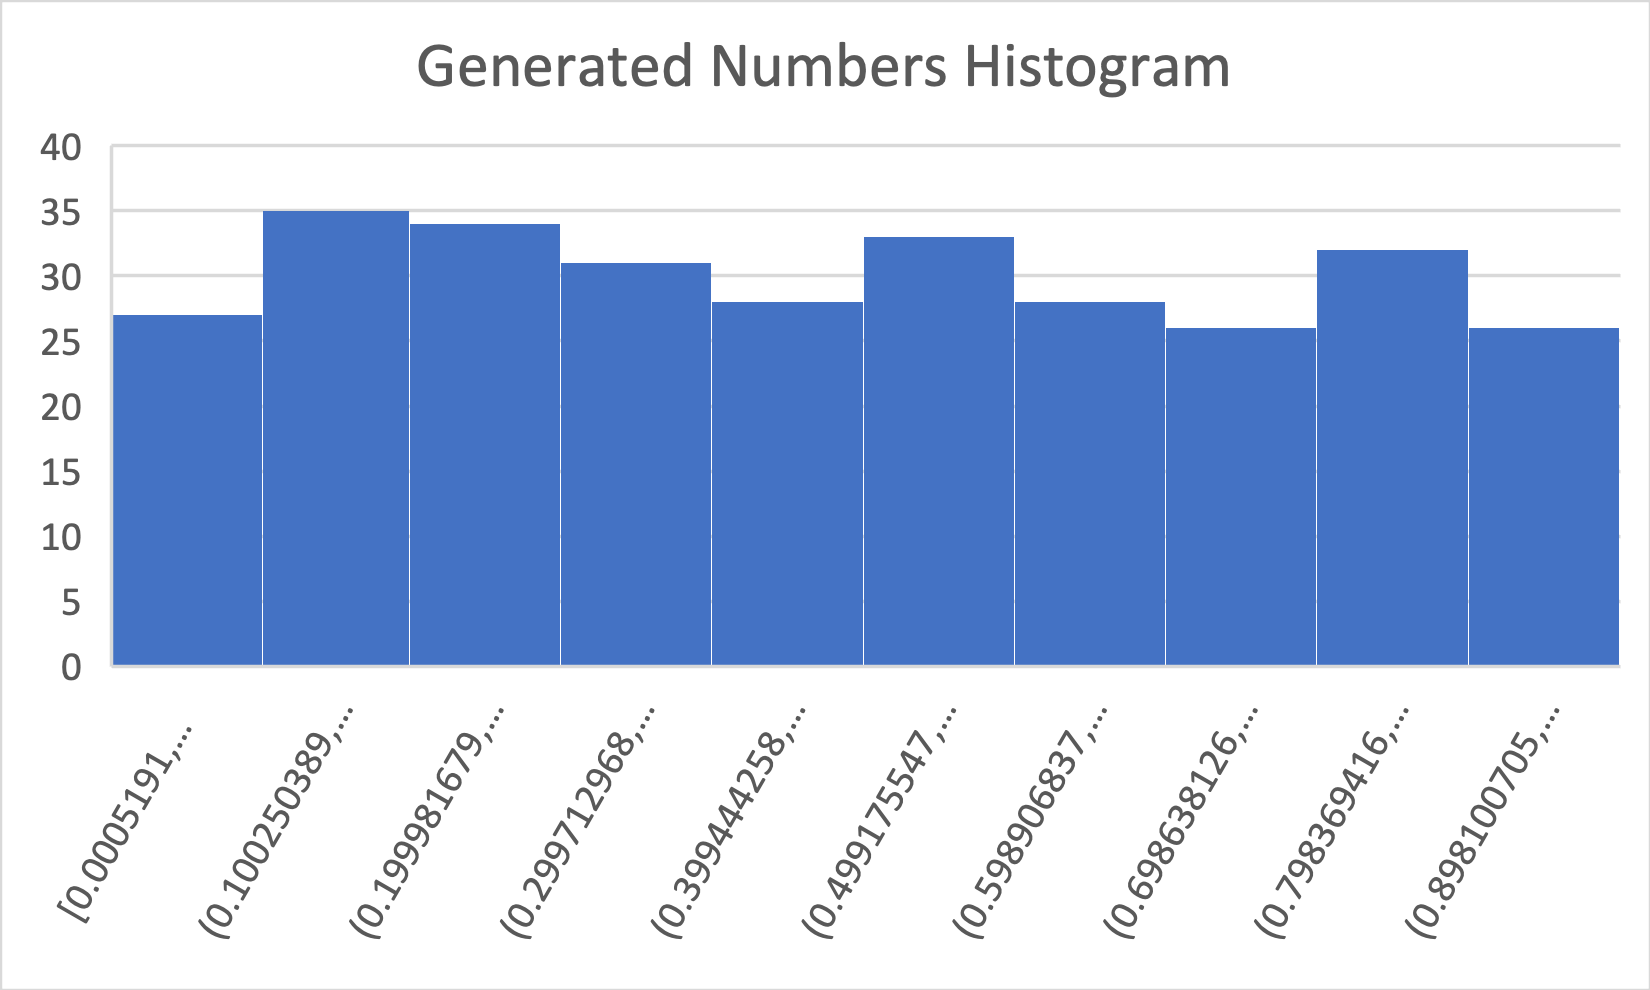
\includegraphics[width=\linewidth]{ranNumGen.png}
        \caption{Generated Number Histogram}
        \label{fig:genNumhisto}
    \end{figure}
    To test for independence an autocorrelation test can be used. I will only complete a single autocorrelation test, but more tests should be done to ensure the generated values are independent. The following formula is used to test for autocorrelation. The value i is the first value tested and the value of m is the lag (autocorrelation between every m number of values generated).
    \clearpage


    % Prints glossaries
    \printglossaries
    % Prints all (used and unused) glossaries 
    \glsaddallunused
    \clearpage
   

    % Prints bibliography
    \printbibliography
    \clearpage


    % Prevents a page number in the toc next to Appendices 
    \noappendicestocpagenum
    % Inserts appendix heading into the toc
    \addappheadtotoc

    % Appendices go below here
    \begin{appendices}
        \section{Extract Data Class}
        \label{app:extractDatapy}
        \begin{code}
            \footnotesize
            \inputminted[linenos=true, fontfamily=courier, autogobble, breaklines, bgcolor=bg]{Python}{./Imports/Code/Extract_Data.py}
            \caption{Extract Data Class}
            \label{lst:extractDatapy}
        \end{code}
        \section{Plot Histograms Class}
        \label{sct:plotHistograms}
        \begin{code}
            \footnotesize
            \inputminted[linenos=true, fontfamily=courier, autogobble, breaklines, bgcolor=bg]{Python}{./Imports/Code/plot_histograms.py}
            \caption{Plot Histograms Class}
            \label{lst:plotHistograms}
        \end{code}
        \section{Q-Q Plots Code}
        \label{sct:qqplotspy}
        \begin{code}
            \footnotesize
            \inputminted[linenos=true, fontfamily=courier, autogobble, breaklines, bgcolor=bg]{Python}{./Imports/Code/plot_QQs.py}
            \caption{Q-Q Plot Code}
            \label{lst:qqplotspy}
        \end{code}
        \section{Random Number Generation Code}
        \label{sct:ranGen}
        \begin{code}
            \footnotesize
            \inputminted[linenos=true, fontfamily=courier, autogobble, breaklines, bgcolor=bg]{Python}{./Imports/Code/RandomNumberGeneration.py}
            \caption{Random Number Generation Code}
            \label{lst:ranNumGen}
        \end{code}
        \clearpage        

    \end{appendices}
    

\end{document}
